\documentclass[../../document.tex]{subfiles}

\begin{document}
    \section{Definite Clause Programs}\label{sec:grammar:dcp}
    \deflab{\dcp}[Definite clause programs]  \defabrv{\dcp}{\abrv{dcp}} were introduced as a formalism to characterize the derivation trees in attribute grammars \citep{Der85}.
    In contrast to \abrv{lcfrs}, it is a formalism where each rule produces trees instead of plain strings.
    The most striking difference to the previous formalism, however, lies in the composition expressions contained in each rule:
    They not only allow substitution with parameters produced by successors in a derivation (first-order substitution), but each single parameter may also contain variables that are substituted in the same step (second-order substitution).
    This corresponds to the information flow from the bottom to the top in a derivation expressed by synthetic attributes (first-order substitution) and the flow from the top to the bottom in a derivation by inherent attributes (second-order substitution) in attribute grammars \citep[cf.\@][Section~1]{Der88}.
    In the implementation of these two systems of substitution, two pairwise distinct sets of variables are used: \(\X\) for the first (as in \abrv{lcfrs}), and \(\Y\) for the second-order substitution.

    In their most general form, the object produced by a derivation in such a \abrv{dcp} is not necessarily computable, as the two types of substitution may mutually recur.
    Some restricted forms that exclude circular dependencies in the expressed productions were introduced to solve this issue \citep[Section~3.4 discusses non-circular attribute grammars]{Cou82}.
    It is easy to see that the definition shown in this section supersedes each of these restricted forms, as it exclusively allows fixed terminal objects or a single second-order variable as a parameter for second-order substitution.
    To avoid unnecessarily complicated definitions, the subset of \abrv{dcp} shown in this section is even further restricted:
    \begin{inparaenum}
        \item Each composition yields one sequence of consecutive trees (and not sequences of ranges) that is a subforest in the parse.
        \item Each rule's composition expression allows exactly one second-order substitution (which may be the empty sequence). Thus, the symbol \(\y\) occurs exactly once in each composition.
    \end{inparaenum}
    We chose both restrictions to avoid having to distinguish successor derivations with special properties for the evaluation of the expressions.

    \begin{definition}[Composition]
        We fix the \(\DN\)-family of finite sets of variables \((\X_k = \{\x_i \mid i \in [k]\} \mid k \in \DN)\), and the singleton set \(\Y = \{\y\}\).
        The identifier \(\X\) denotes the set of all variables \(\X = \{\x_i \mid i \in \DN\}\).
        Let \(\varSigma\) and \(\varGamma\) be alphabets disjoint from \(\X \cup \Y\).
        The \(\DN\)-family \((S_k = \{x(v) \mid x \in \X_k, v \in \T_\varGamma(\varSigma \cup Y)^*\} \mid k \in \DN)\) denotes substitution sites with variables up to subscript \(k\).
        The \(\DN\)-family of \abrv{dcp} \deflab<composition>{\abrv{dcp} composition}[compositions] over \(\varSigma\) and \(\varGamma\) is \((\C^{\varGamma\varSigma}_k \mid k \in \DN)\) such that \(\C^{\varGamma\varSigma}_k\) contains each nonempty sequence \(c\) in \((\T_\varGamma(\varSigma \cup \Y \cup S_k))^+\) such that each variable in \(\X_k \cup \Y\) occurs exactly once in \(c\).
        The identifier \(\C^{\varGamma\varSigma}\) denotes the set of all \abrv{dcp} compositions \(\bigcup_{k \in \DN} \C^{\varGamma\varSigma}_{k}\).

        Each composition \(c \in \C^{\varGamma\varSigma}_k\) is associated with a function \[
            \sem{c}\colon \big(\T_\varGamma(\varSigma \cup Y)^*\big)^k \to \T_\varGamma(\varSigma \cup Y)^*
        \] that is defined as follows:
            Let \((\x_i(w_i) \in S_k \mid i \in [k])\) be the family of substitution sites occurring in \(c\) and \((v_i \in \T_\varGamma(\varSigma \cup Y)^* \mid i \in [k])\) a family of arguments.
            Then \(\sem{c}\) is defined as a second-order substitution of \(\X_k\) in \(c\) such that \(\sem{c}(\xi_1, \ldots, \xi_k) = c\big[\x_1(w_1)=\xi_1[\y=w_1], \ldots, \x_k(w_k)=\xi_k[\y=w_k]\big]\).
    \end{definition}

    %    The occurrences of variables are abbreviated in the following two ways:
    %    \begin{compactenum}
        %        \item Variables in \(\X\) with successor \(\varepsilon\) are abbreviated by omitting the parentheses and the successor as a whole; e.g.\@ instead of \(\x_1(\varepsilon)\), we just write \(\x_1\).
        %        \item We omit trailing occurrences of the variable \(\y\) if it does not occur as a successor of any node; e.g.\@ instead of \(\text{S}(\x_1)\,\y \), we just write \(\text{S}(\x_1)\).
        %    \end{compactenum}

    \begin{example}\label{ex:dcp:comp}
        Consider the following six \abrv{dcp} compositions over the two alphabets \(\varGamma = \{ \cn{sbar}, \cn{s}, \cn{vp}, \cn{np} \}\) and \(\varSigma = \{\tn{where}, \tn{the}, \tn{survey}, \tn{was}, \tn{carried}, \tn{out}\}\):
        \begin{align*}
            c_1 &= \tn{where} \, \y,
            &c_2 &= \y \, \tn{out},
            &c_3 &= \cn{np} (\y \, \tn{survey}) && \in \C_0\\
            c_4 &= \cn{vp}(\x_1(\y) \, \tn{was}) && && && \in \C_1 \\
            c_5 &= \cn{sbar} (\cn{s} (\x_1(\y) \, \x_2(\tn{the}))),
            &c_6 &= \cn{vp}(\x_1(\y) \, \x_2(\tn{carried})) && && \in \C_2
        \end{align*}
        The subscript in the family of \abrv{dcp} compositions \(\C^{\varGamma\varSigma}\) determines the number of arguments for the functions represented by the elements in \(\C\).
        E.g.\@ \(\sem{c_1}\) takes no arguments, and \(\sem{c_6}\) takes two arguments.
        Evaluating any term of these compositions yields a sequence tree in \(\T_\varGamma(\varSigma \cup \Y)\) with exactly one occurrence of \(\y\), for example:
        \begin{align*}
            \sem{c_6} \big( \sem{c_1}(), \sem{c_2}() \big)
            &= \sem{c_6} \big( \: (\tn{where} \, \y), \: (\y \, \tn{out}) \: \big) \\
            &= \cn{vp}(\x_1(\y) \, \x_2(\tn{carried}))[\x_1(\y)=(\tn{where} \, \y), \x_2(\tn{carried})=(\tn{carried}\, \tn{out})] \\
            &= \cn{vp}(\tn{where} \, \y \, \tn{carried out})
        \end{align*}
    \end{example}

    Aside from the form of the compositions (and therefore also the concept of fanout), \abrv{dcp} grammars, \deflab<derivation>{\abrv{dcp} derivation}[derivations], and most of the concepts of rule and grammar forms are defined analogously to \abrv{lcfrs} grammars, and we will refrain from repeating them completely but focus on the differences to \abrv{lcfrs} grammars.
    As we have seen, \abrv{dcp} compositions contain elements from two alphabets, \(\varGamma\) for inner nodes (which we will assume to be constituent symbols) and  \(\varSigma\) for leaf nodes (tokens or sentence positions, respectively), only the symbols in \(\varSigma\) are considered lexical symbols.
    The tuple for a \abrv{dcp} grammar is hence extended by the additional alphabet and assumes the form \((N, \varGamma, \varSigma, S, R)\).
    There is no fanout in \abrv{dcp} because the sequences of trees produced by compositions are not meant to be separated.
    To avoid that a complete derivation produces more than one tree, we require that the composition in each non-nullary rule whose \abrv{lhs} nonterminal is an initial nonterminal in \(S\) is of the form \(\gamma ( \omega )\) for some \(\gamma \in \varGamma\) and \(\omega \in \C^{\varGamma \varSigma}\), i.e.\@ there is at least one inner node that assembles the results of all successor rules.
    As in other grammar formalisms, the yield for a derivation recursively computes the composition functions.
    This recursive evaluation will leave exactly one superfluous variable symbol \(\y\) that originates from the root's composition; it is removed from the result.
    In contrast to string grammars, like \abrv{lcfrs}, the \deflab<yield>{yield of a \abrv{dcp} derivation}[yield] of a complete derivation is a tree in \(\T_\varGamma(\varGamma)\).

    As \abrv{lcfrs}, we deal with \abrv{dcp} grammars that are instantiated with sentence positions as lexical symbols during the rule extraction as well as parsing.
    The formalism does not restrict the composition functions with respect to the lexical symbols of assembled trees; each derivation is inherently \deflab<admissible>{admissible \abrv{dcp} derivation}[admissible].\footnote{
        Such ``unrestricted \abrv{dcp}'' showed to be infeasible for parsing during our experiments, so we equipped each rule with a fanout (which does not need to be consistent among all rules for a \abrv{lhs} nonterminal).
        This is discussed in more detail in \cref{sec:supertags,sec:parsing:dcp}.
    }
    For each derivation \(d\) in a position instantiated \abrv{dcp}, the constituent structure for \(d\) is the yield of \(d\).

    \begin{example}[Continues \cref{ex:dcp:comp}]\NoEndMark
        Consider a \abrv{dcp} \((N, \varGamma, [|w|], \nt{s}, R)\) that is a position instantiation for \(w = \text{``where the survey was carried out''}\), with the alphabets \(N = \{\nt{v}^\nt{L}, \nt{v}, \nt{n}, \nt{s} \}\) and \(\varGamma = \{\cn{vp}, \cn{sbar}, \cn{s}, \cn{np}\}\), and
        \begin{align*}
            R = \Big\{ \quad
            \nt{v}^\nt{L} &\to (\tn{1} \, \y)\:(),
            \quad \nt{v} \to (\y \, \tn{6})\:(),
            &\nt{n} &\to (\cn{np} (\y \, \tn{3}))\:(), \\
            \nt{v} &\to (\cn{vp}(\x_1(\y) \, \tn{4}))\:(\nt{v}),  \\
            \nt{s} &\to (\cn{sbar} (\cn{s} (\x_1(\y) \, \x_2(\tn{2}))))\:(\nt{v}, \nt{n}),
            &\nt{v} &\to (\cn{vp}(\x_1(\y) \, \x_2(\tn{5})))\:(\nt{v}^\nt{L}, \nt{v})
            \quad \Big\} \text{.}
        \end{align*}

        The tree \(d\) illustrated below (left) is a derivation in \(\derivs^R_\nt{s}\), its constituent structure \(\yield(d)\) is shown to the right.
        A part of the computations (for the bottom \(\cn{vp}\)-node) was already shown in the previous example in detail.

        \null\hfill
        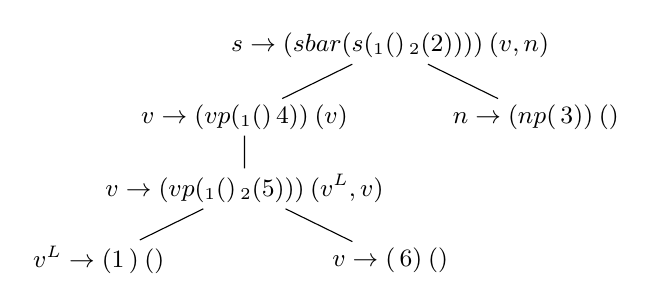
\begin{tikzpicture}[level distance=6ex, font=\small, sibling distance=3.7cm, inner sep=2pt]
            \node {\(\nt{s} \to (\cn{sbar} (\cn{s} (\x_1(\y) \, \x_2(\tn{2}))))\:(\nt{v}, \nt{n})\)}
                child {node {\(\nt{v} \to (\cn{vp}(\x_1(\y) \, \tn{4}))\:(\nt{v})\)}
                    child {node {\(\nt{v} \to (\cn{vp}(\x_1(\y) \, \x_2(\tn{5})))\:(\nt{v}^\nt{L}, \nt{v})\)}
                        child {node {\(\nt{v}^\nt{L} \to (\tn{1} \, \y)\:()\)}}
                        child {node {\(\nt{v} \to (\y \, \tn{6})\:()\)}}}}
                child {node {\(\nt{n} \to (\cn{np} (\y \, \tn{3}))\:()\)}};
        \end{tikzpicture}
        \hfill
        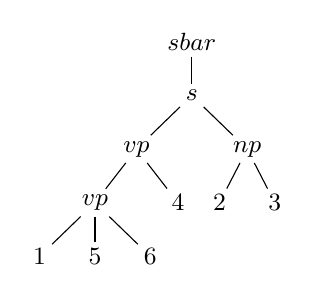
\begin{tikzpicture}[level distance=4.5ex, font=\small, inner sep=2pt, sibling distance=4em]
            \node {\(\cn{sbar}\)} child {node {\(\cn{s}\)}
                child {node {\(\cn{vp}\)}
                    [sibling distance=3em]
                    child {node {\(\cn{vp}\)}
                        [sibling distance=2em]
                        child {node {\(\tn{1}\)}}
                        child {node {\(\tn{5}\)}}
                        child {node {\(\tn{6}\)}}}
                    child {node {\(\tn{4}\)}}}
                child {node {\(\cn{np}\)}
                    [sibling distance=2em]
                    child {node {\(\tn{2}\)}}
                    child {node {\(\tn{3}\)}}}};
        \end{tikzpicture}
        \hfill\exampleqed{}
    \end{example}

    The following definition is used for the extraction of \abrv{dcp} compositions from an indexed tree.
    It identifies a coherent set of positions in the input tree using a sequence of parallel (bottom) positions and a common ancestor.
    Each position is complemented with a set of leaves to accomodate missing elements that are represented by second-order substitution sites.

    \begin{definition}\label{def:dcp:comp}
        Consider an indexed tree \(\xi \in \itrees_{\varSigma}\) over any alphabet \(\varSigma\) together with
        \begin{itemize}
            \item
                a collection of \(k \in \DN\) parallel positions \((\rho_i \in \pos(\xi) \mid i \in [k])\) and
                a common ancestor position \(\rho_0 \in \bigcap_{i \in [k]} \ancestors(\rho_i)\), as well as
            \item
                a non-empty set of leaves \((L_i \subseteq \yield(\xi|_{\rho_i}) \mid i \in [0, k])\) for each such position such that
                \(L_0\) subsumes all other sets: \(\bigcup_{i\in[k]} L_i \subseteq L_0\). Additionally, \(L_i\) must differ at most by one leaf from the set of leaves \(\yield(\xi|_{\rho_i})\) for each \(i \in [0,k]\).
        \end{itemize}

        The \abrv{dcp} composition \(c \in \C^\varSigma_k\) for \(\xi\) and \(((\rho_i, L_i) \mid i \in [0,k])\) is defined as follows:
        \begin{itemize}
            \item
                the occurrences for second-order substitution are either of the form \(\omega_i = \ell_i\) if the set \(\yield(\xi|_{\rho_i}) \setminus L_i = \{\ell_i\}\) is a singleton and otherwise \(\omega_i = \varepsilon\) for each \(i \in [k]\),
            \item
                \(c'\) is obtained from \(\xi|_{\rho_0}\) be replacing the subtree at position
                \(\rho_i\) with \(\x_i(\omega_i)\) for each \(i \in [k]\), and
            \item
                if \(\yield(\xi|_{\rho_0}) \setminus L_0 = \{\ell_0\}\) is a singleton set,
                then \(c\) is obtained from \(c'\) by replacing \(\ell_0\) by the variable\(\y\), otherwise \(c = c' \, \y\).
        \end{itemize}
        We denote \(c\) by \(\mathrm{scomp}(\xi, (\rho_0, L_0), (\rho_1, L_1), \ldots, (\rho_k, L_k))\).
    \end{definition}

    \begin{example}\NoEndMark
        Consider the indexed tree \(\xi\) below and the positions marked at its root \(\rho_0 = \varepsilon\) as well as at its grandchildren \(\rho_1 = 1\,1\) and \(\rho_2=1\,2\).
        Moreover consider the three sets of leaves \(L_0 = \yield(\xi) = [6]\), \(L_1 = \yield(\xi|_{\rho_1}) = \{1,4,5,6\}\) and \(L_2 = \{3\} = \yield(\xi|_{\rho_2}) \setminus \{2\}\); note that \(L_0 = L_1 \cup L_2 \cup \{2\}\).
        The composition \(\mathrm{scomp}(\xi, (\rho_0, L_0), (\rho_1, L_1), (\rho_2, L_2))\) is obtained as follows:
        \begin{itemize}
            \item  we define two arguments for second-order substitution, \(\omega_1 = \varepsilon\) since \(L_1 = \yield(\xi|_{\rho_1})\), and \(\omega_2 = 2\) since \(L_2 = \yield(\xi|_{\rho_2}) \setminus \{2\}\);
            \item \(c'\) consists of the nodes in \(\xi\) starting with the root \(\rho_0 = \varepsilon\) to the bottom up to the positions \(\rho_1\) and \(\rho_2\) which are replaced by the variables \(\x_1\) and \(\x_2\) extended by the parameters \(\omega_1\) and \(\omega_2\), it is \(c' = \cn{sbar}(\cn{s} (\x_1(\varepsilon), \x_2(2)))\),
            \item the composition \(c\) is \(c'\) extended by a trailing occurrence of the variable \(\y\), since \(L_0 = \yield(\xi_{\rho_0})\), hence \(\mathrm{scomp}(\xi, (\rho_0, L_0), (\rho_1, L_1), (\rho_2, L_2)) = \cn{sbar}(\cn{s} (\x_1(\varepsilon), \x_2(2))) \, \y\).
        \end{itemize}
 
        \null\hfill
        \begin{tikzpicture}[level distance=4.5ex, font=\small, inner sep=2pt, sibling distance=4em, baseline=(bottom.base)]
            \node (root) {\strut{}\(\cn{sbar}\)} child {node {\(\cn{s}\)}
                child {node (vp1) {\(\cn{vp}\)}
                    [sibling distance=3em]
                    child {node {\(\cn{vp}\)}
                        [sibling distance=2em]
                        child {node (bottom) {\(\tn{1}\)}}
                        child {node {\(\tn{5}\)}}
                        child {node {\(\tn{6}\)}}}
                    child {node {\(\tn{4}\)}}}
                child {node (np) {\(\cn{np}\)}
                    [sibling distance=2em]
                    child {node (t2) {\(\tn{2}\)}}
                    child {node {\(\tn{3}\)}}}};
            \node[gray, left=0.1cm of root] {$\rho_0$};
            \node[gray, right=0.1cm of vp1] {$\rho_1$};
            \node[gray, right=0.1cm of np] {$\rho_2$};
            % \node[fit=(t2), gray, circle, draw] {\phantom{\tn{2}}};
            \node[left=1cm of vp1] {$\xi = $}; 
        \end{tikzpicture}
        \hfill
        \begin{tikzpicture}[level distance=4.5ex, font=\small, inner sep=2pt, sibling distance=4em, baseline=(bottom.base)]
            \node (root) {\strut{}\(\cn{sbar}\)}
                child {node (s) {\(\cn{s}\)}
                    child {node (vp1) {\(\x_1(\varepsilon)\)}}
                    child {node (np) {\(\x_2(2)\)}
                     child{node {\phantom{\cn{vp}}} edge from parent[draw=none]
                        child{node (bottom) {\phantom{\cn{1}}}  edge from parent[draw=none]}}}};
            \node[right=.3cm of root] (vy) {\strut{}\(\y\)};
            \node[left=1cm of s] {$c=$}; 
        \end{tikzpicture}
        \hfill\exampleqed
    \end{example}

    \begin{lemma}
        Let \(\xi \in \itrees_{\varSigma}\), \(k \in \DN\) and \(((\rho_i, L_i) \in \pos(\xi) \times \power(\yield({\xi})) \mid i \in [0,k])\) be an indexed tree, positions and sets of leaves as specified in \cref{def:dcp:comp}.
        Moreover, let \((\xi_i' \in \T_\varSigma(\DN_+ \cup \{\y\}) \mid i \in [0,k])\) be trees such that, for each \(i \in [0,k]\) the tree \(\xi_i'\) is obtained from \(\xi|_{\rho_i}\) as follows:
        \begin{compactitem}
            \item if \(\yield(\xi|_{\rho_i}) \neq L_i\), then by replacing each leaf in \(\yield(\xi|_{\rho_i}) \setminus L_i\) by the variable \(\y\) (there is at most one such leaf),
            \item otherwise by adding a trailing variable \(\y\) such that \(\xi_i' = \xi_{\rho_i}\,\y\).
        \end{compactitem}
        
        Then \(\sem{\mathrm{scomp}(\xi, (\rho_0, L_0), (\rho_1, L_1), \ldots, (\rho_k, L_k))}(\xi_1', \ldots, \xi_k') = \xi_0'\).
        % The composition \(c = \mathrm{scomp}(\xi, (\rho_0, L_0), (\rho_1, L_1), \ldots, (\rho_k, L_k))\) is defined such that \(\xi_0' = \sem{c}(\xi_1', \ldots, \xi_k')\) where each tree \(\xi_i'\) is \(\xi|_{\rho_i}\) but if \(\yield(\xi|_{\rho_i}) \neq L_i\) then the leaf in the difference \(\yield(\xi|_{\rho_i}) \setminus L_i\) is replaced by \(\y\).
    \end{lemma}
\end{document}